\section{Visão dos clientes e comparativos}

clientes: mari, hugo, caelum

Metodologias

XP
Lean
Scrum
Crystal


Antes de iniciar o desenvolvimento do Calopsita, resolvemos analisar quais seriam as outras alternativas disponíveis no mercado. Fizemos uma análise bem extensa, tanto de produtos pagos, quanto de livres e \opensource. A idéia era descobrir quais os pontos fortes de cada ferramenta, e implementá-los no Calopsita. Embora as ferramentas pagas não sejam exatamente concorrentes, mostrar que nosso sistema tem as mesmas ou mais funcionalidades que as alternativas pagas, pode fazer com que atraiamos mais usuários e colaboradores.

\begin{itemize}
\item Scrumy - https://scrumy.com/
pago / proprietario
interface baseada em drag and drop
leve
nao é customizavel
snapshots do projeto no passado e futuro (board image)
live update
nao permite estimativas
nao permite marcacao horas
nao trabalha com templates nem personas
burndown

\begin{figure}[H]
  \centering
  \fbox{
    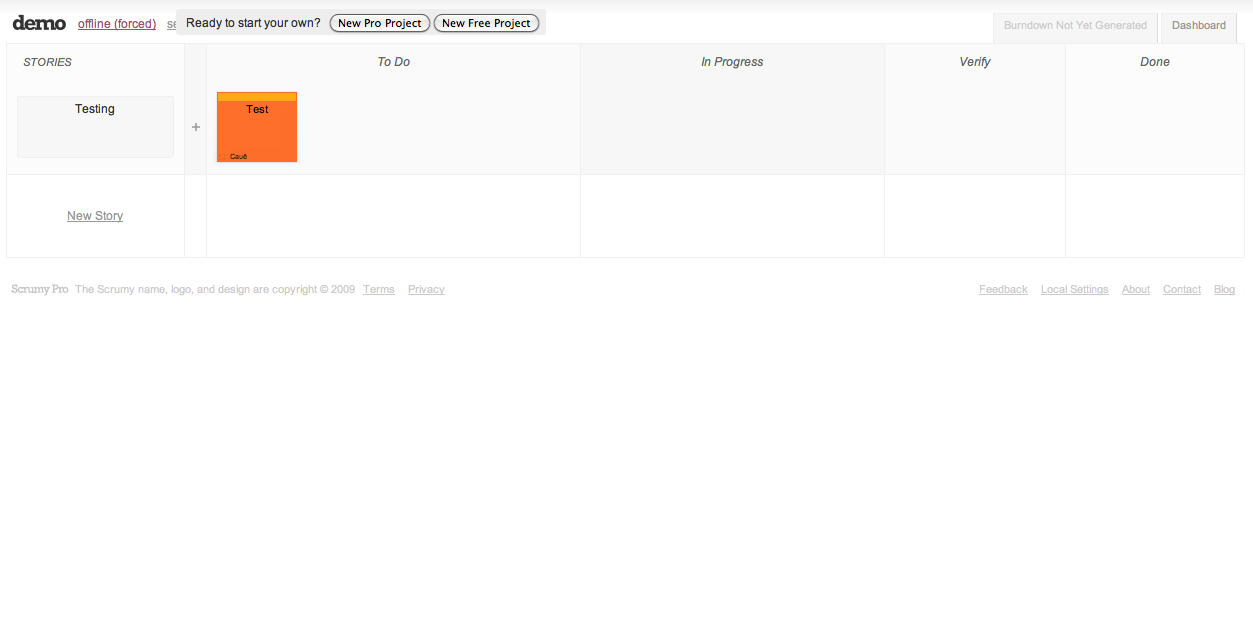
\includegraphics[width=110mm]{images/scrumy_1.png}
  }
  \caption{Scrumy - kanban}
\end{figure}

\item ScrumNinja - http://scrumninja.com
pago / proprietario
pouco customizavel
estimativa (1, 2 ou 3)
interface baseada em estados (start, deliver, etc)
leve
graficos de progresso
sem marcacao de horas
nao trabalha com templates nem personas
API para atualizar

\begin{figure}[H]
  \centering
  \fbox{
    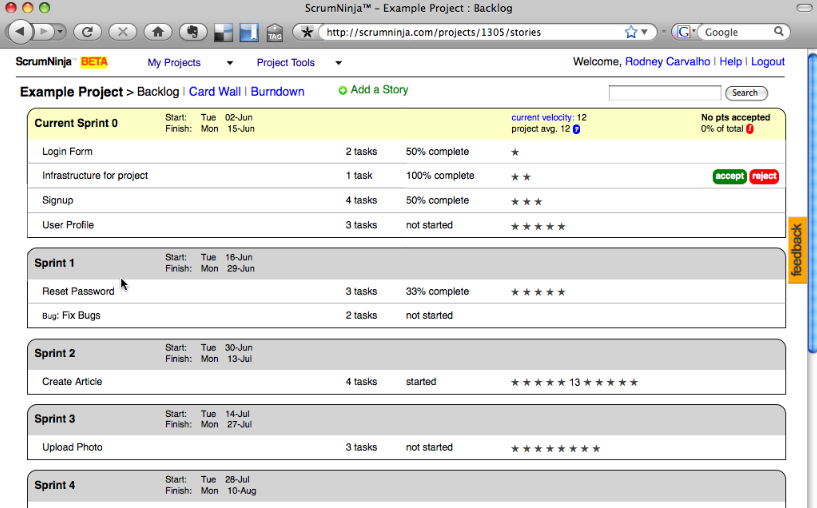
\includegraphics[width=110mm]{images/scrum_ninja_1.png}
  }
  \caption{ScrumNinja - kabacklognban}
\end{figure}

\begin{figure}[H]
  \centering
  \fbox{
    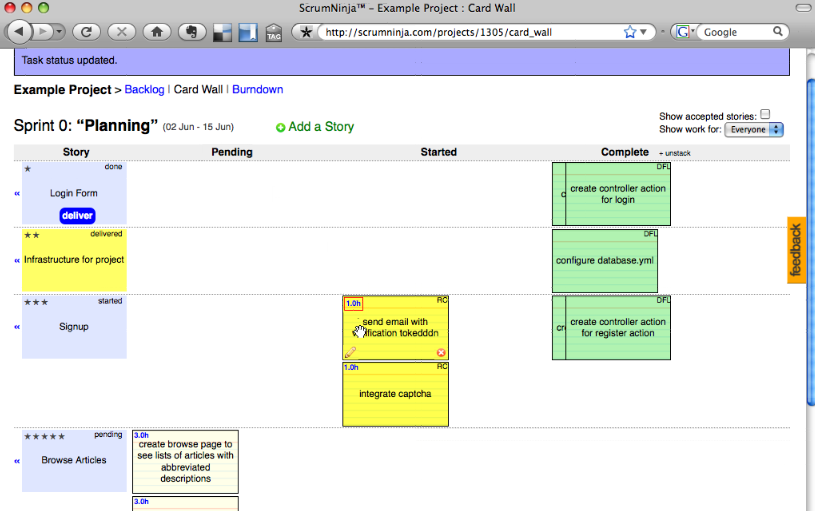
\includegraphics[width=110mm]{images/scrum_ninja_2.png}
  }
  \caption{ScrumNinja - kanban}
\end{figure}

\begin{figure}[H]
  \centering
  \fbox{
    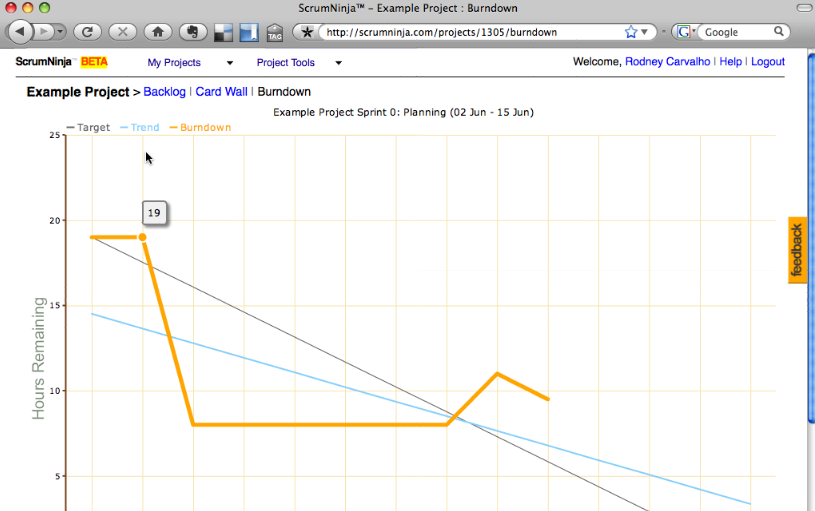
\includegraphics[width=110mm]{images/scrum_ninja_3.png}
  }
  \caption{ScrumNinja - burndown}
\end{figure}

\item scrum'd - http://scrumd.com/
pago / proprietario
nao customizavel
estorias estimadas em pontos
tarefas estimadas em horas
burndown
import/export tarefas e estorias
nao trabalha com templates nem personas

\begin{figure}[H]
  \centering
  \fbox{
    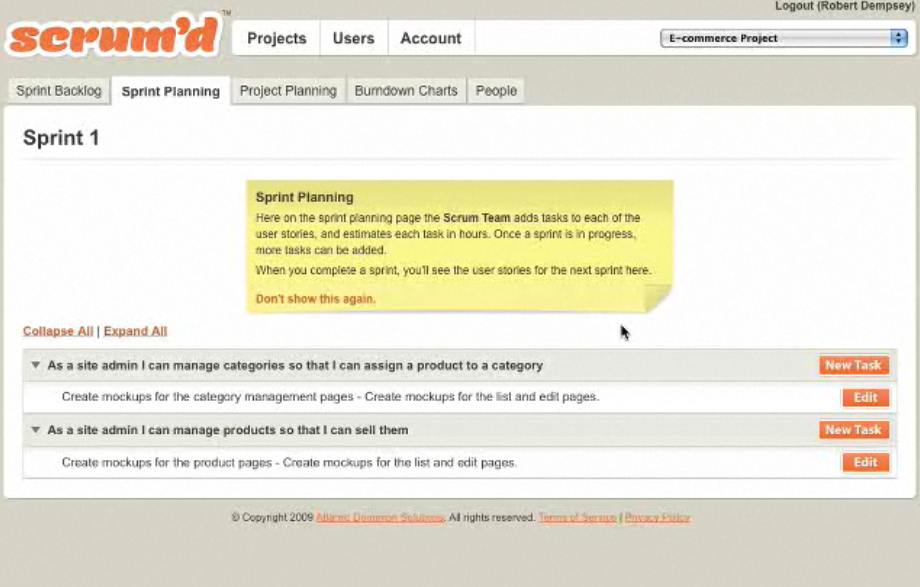
\includegraphics[width=110mm]{images/scrumd.png}
  }
  \caption{Scrum'd - sprint planning}
\end{figure}

\item Pivotal Tracker - http://www.pivotaltracker.com/
gratuito / proprietario
import/export tarefas e estorias
classificacao de estoria em bug/feature/chore/release
estimativa (1, 2 ou 3)
nao trabalha com templates nem personas
estados
marcacao de velocidade

\begin{figure}[H]
  \centering
  \fbox{
    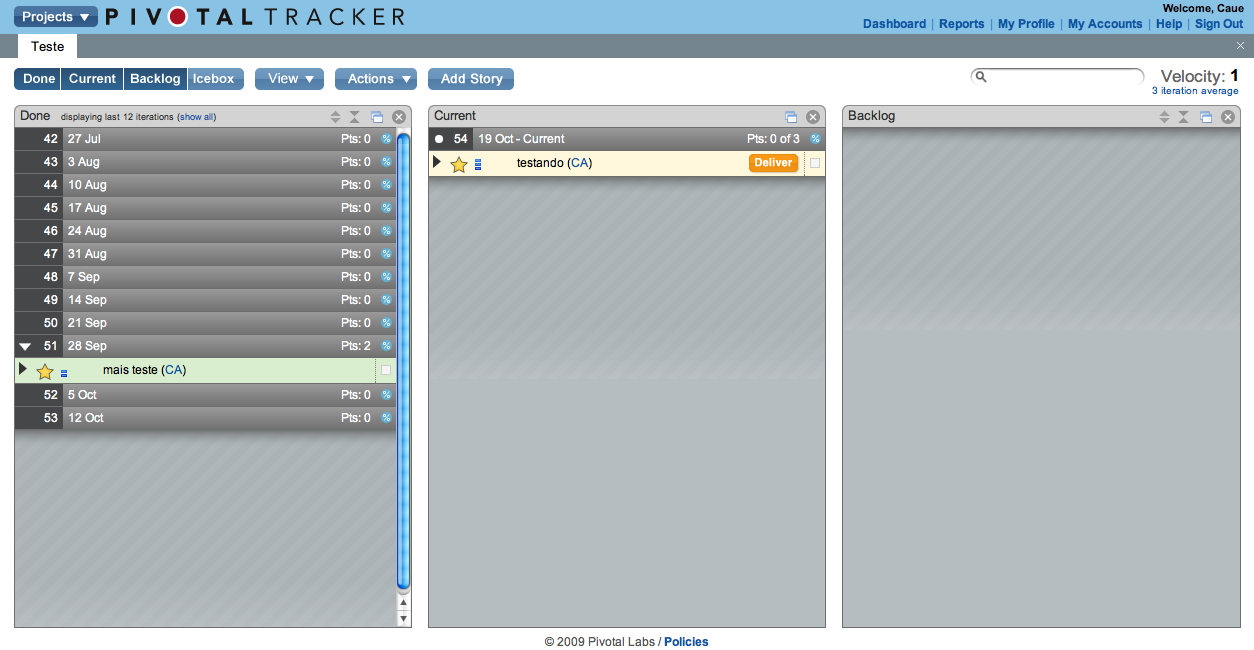
\includegraphics[width=110mm]{images/pivotal_tracker.png}
  }
  \caption{pivotal tracker - kanban}
\end{figure}

\item XPlanner - xplanner.org/
free/open source
nao trabalha com templates nem personas
graficos
estimativas
marcação de horas
nao customizavel

\begin{figure}[H]
  \centering
  \fbox{
    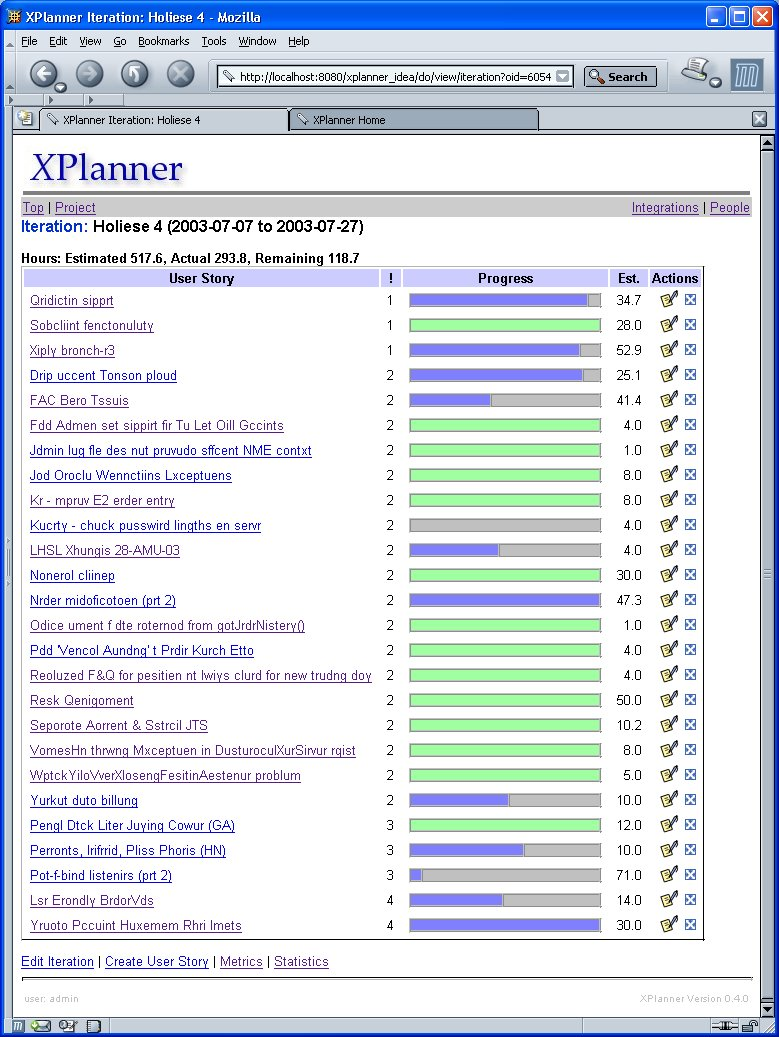
\includegraphics[width=110mm]{images/xplanner.jpg}
  }
  \caption{xplanner - kanban}
\end{figure}

\item VersionOne - http://www.versionone.com
**varias metodologias**
customizavel
burndown
velocidade
planejamento releases
nao trabalha com templates nem personas

\begin{figure}[H]
  \centering
  \fbox{
    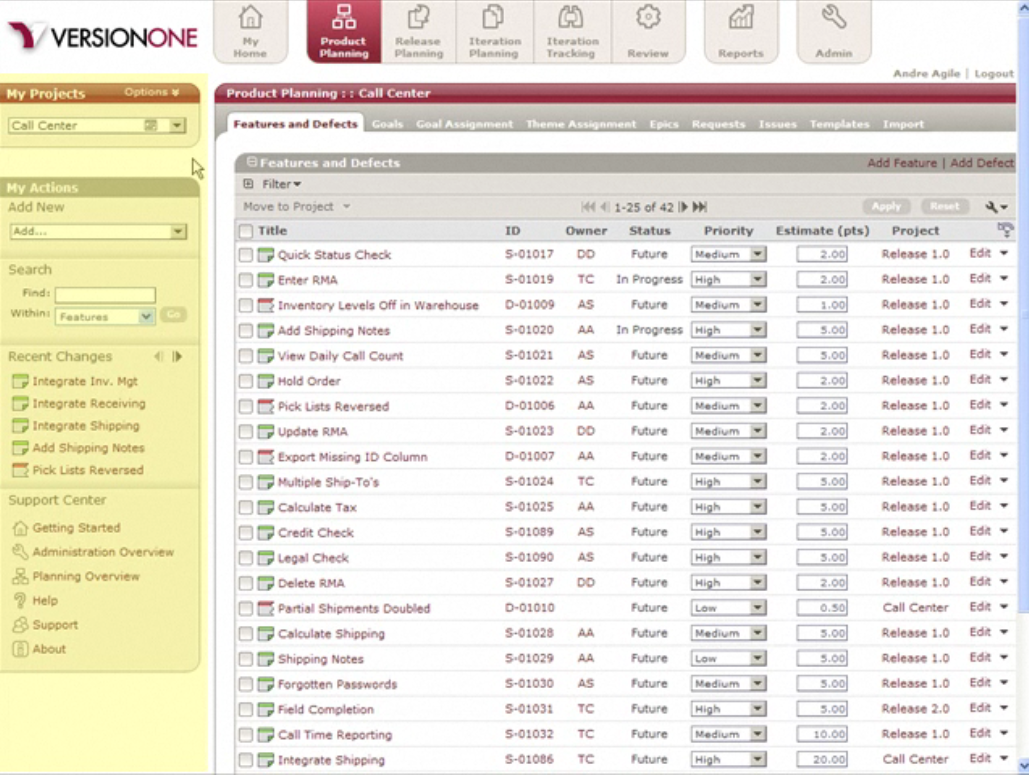
\includegraphics[width=110mm]{images/version_one_1.png}
  }
  \caption{version one - kanban}
\end{figure}

\begin{figure}[H]
  \centering
  \fbox{
    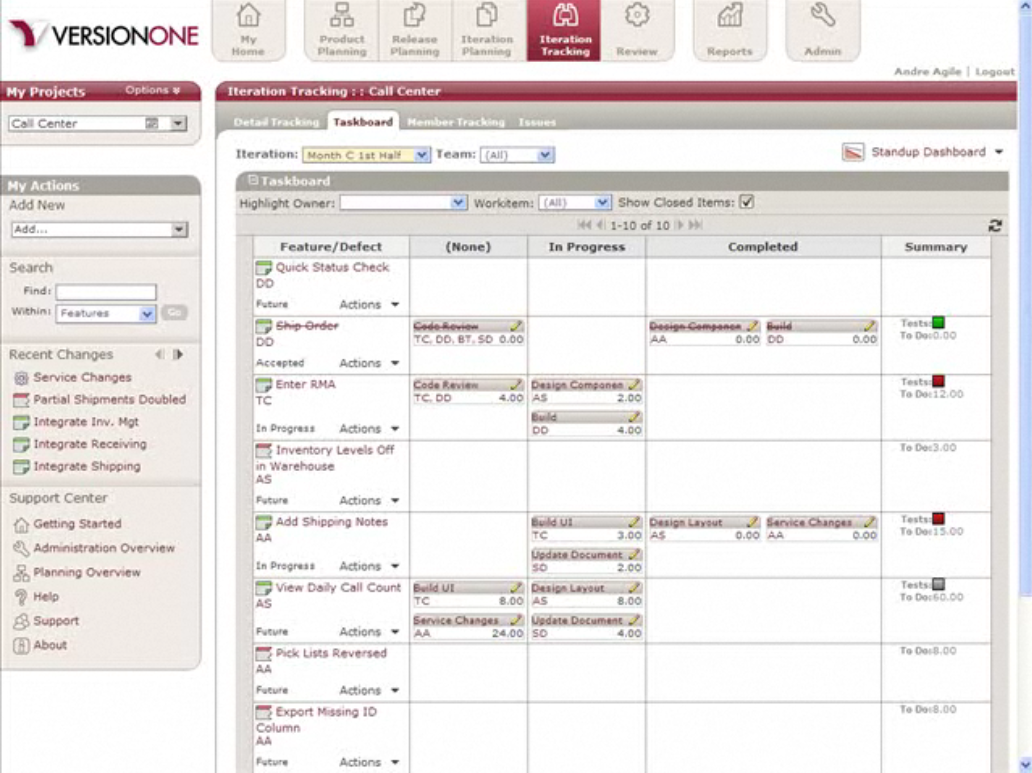
\includegraphics[width=110mm]{images/version_one_2.png}
  }
  \caption{version one - kanban}
\end{figure}

\begin{figure}[H]
  \centering
  \fbox{
    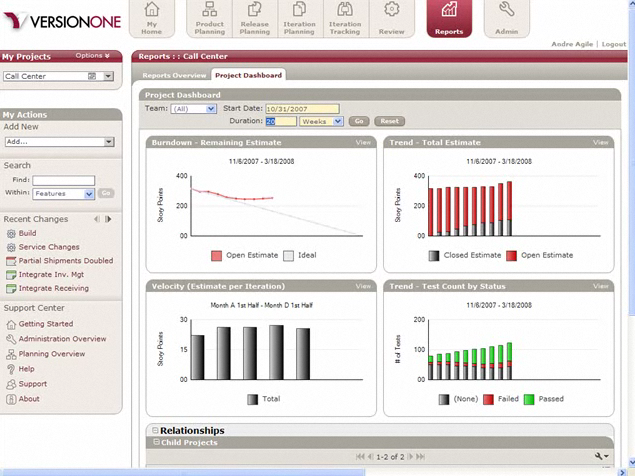
\includegraphics[width=110mm]{images/version_one_3.png}
  }
  \caption{version one - kanban}
\end{figure}

\begin{figure}[H]
  \centering
  \fbox{
    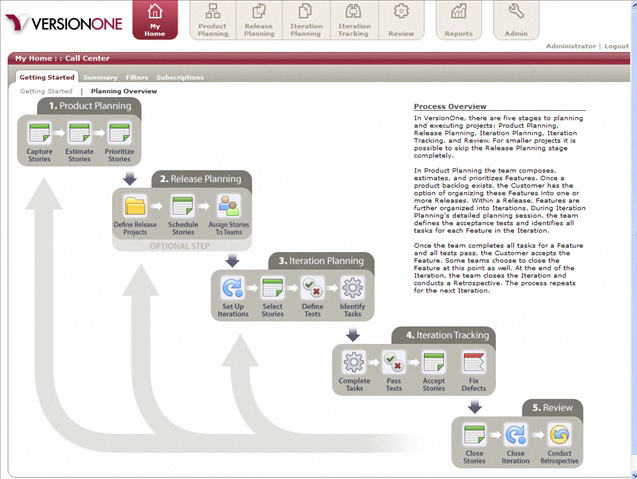
\includegraphics[width=110mm]{images/version_one_4.png}
  }
  \caption{version one - kanban}
\end{figure}

\item Pronto - http://www.bluesoft.com.br/pronto-demo
usuarios com perfis diferentes (po, sm, dev, test, support)
burndown com problemas
priorizacao
lançamento de esforço
informação sobre se foi pareio
sem templates nem personas
nao customizavel
codigo fonte em portugues
livre / open source (github)

\begin{figure}[H]
  \centering
  \fbox{
    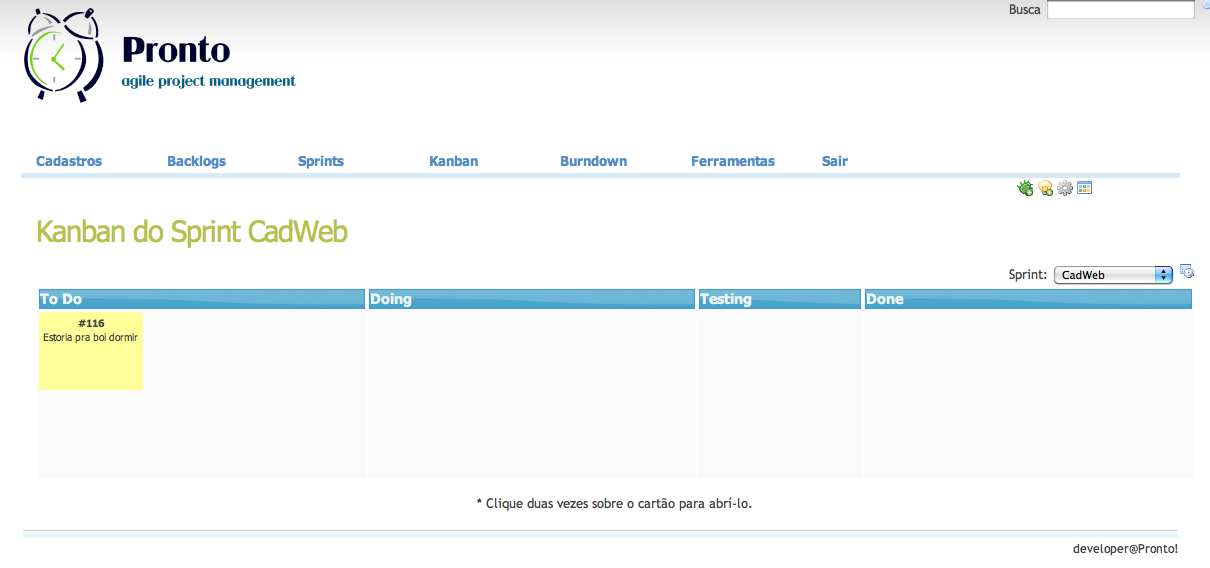
\includegraphics[width=110mm]{images/blue_soft_pronto_1.png}
  }
  \caption{pronto}
\end{figure}

\begin{figure}[H]
  \centering
  \fbox{
    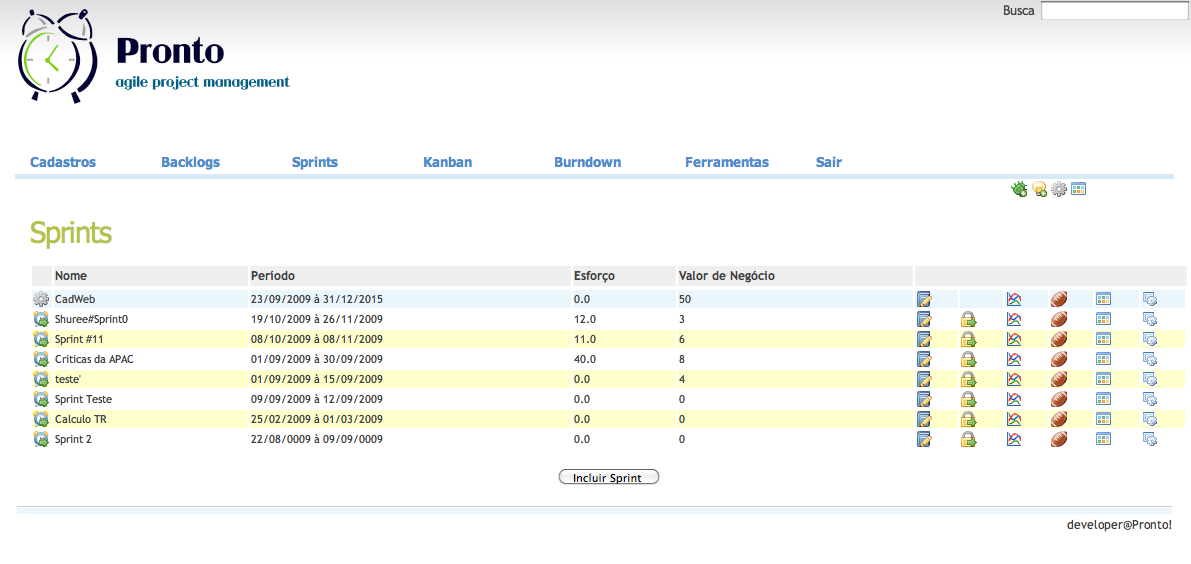
\includegraphics[width=110mm]{images/blue_soft_pronto_2.png}
  }
  \caption{pronto}
\end{figure}

\begin{figure}[H]
  \centering
  \fbox{
    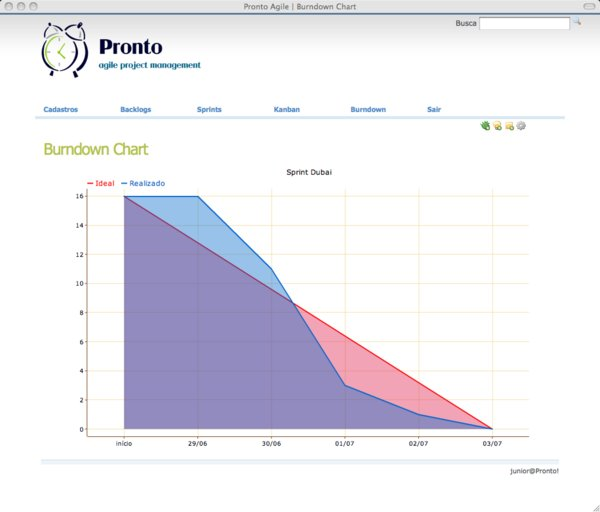
\includegraphics[width=110mm]{images/blue_soft_pronto_3.jpg}
  }
  \caption{pronto}
\end{figure}

\item PPTS - http://ses-ppts.sourceforge.net/
free/open source
prioritizacao
burndown / graficos
velocidade / estimativas
controle de tarefas por pessoas
customização de menus
sem templates nem personas

\begin{figure}[H]
  \centering
  \fbox{
    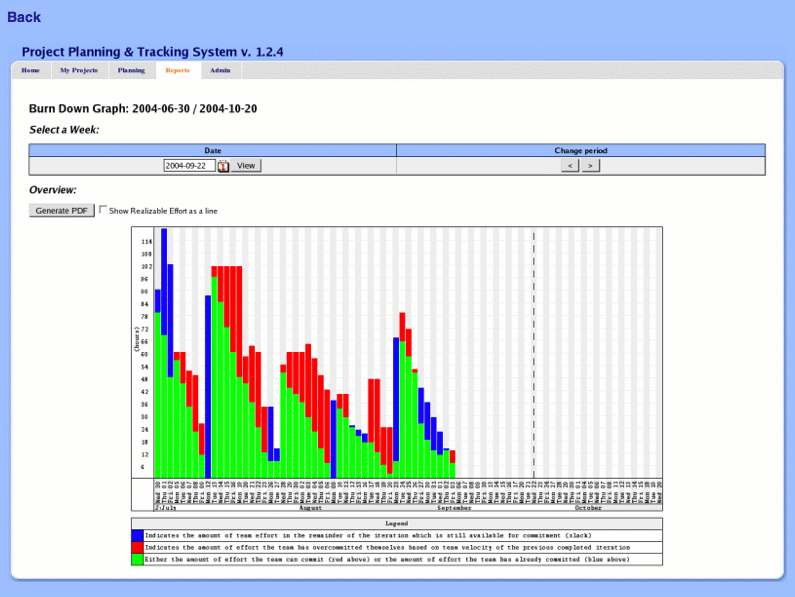
\includegraphics[width=110mm]{images/ppts_1.png}
  }
  \caption{PPTS}
\end{figure}

\begin{figure}[H]
  \centering
  \fbox{
    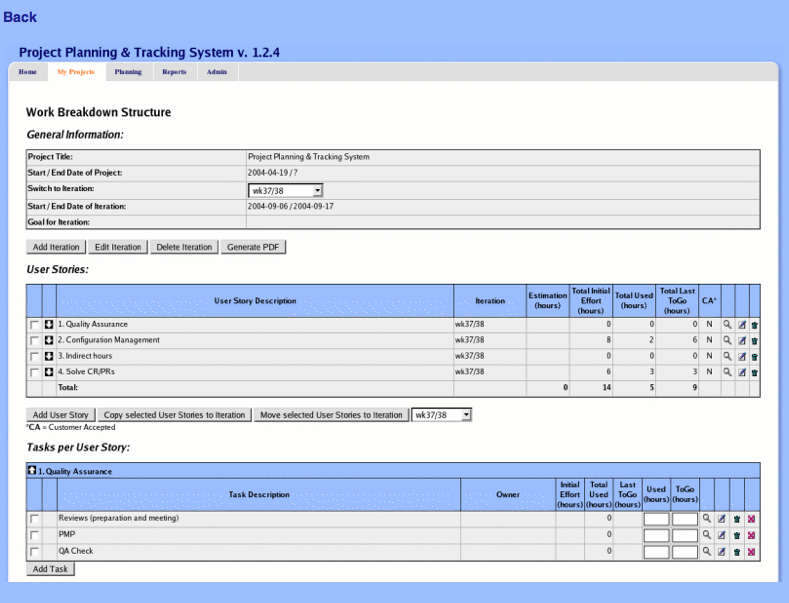
\includegraphics[width=110mm]{images/ppts_2.png}
  }
  \caption{PPTS}
\end{figure}

\item AgileTrac - http://www.agile-trac.org
sistema de tickets
free/open source
sem graficos
sem customizações
apenas abas de iterações e backlog
medida de tamanha por pontos
acompanhamento de progresso por barra de percentagem x percento pronto

\begin{figure}[H]
  \centering
  \fbox{
    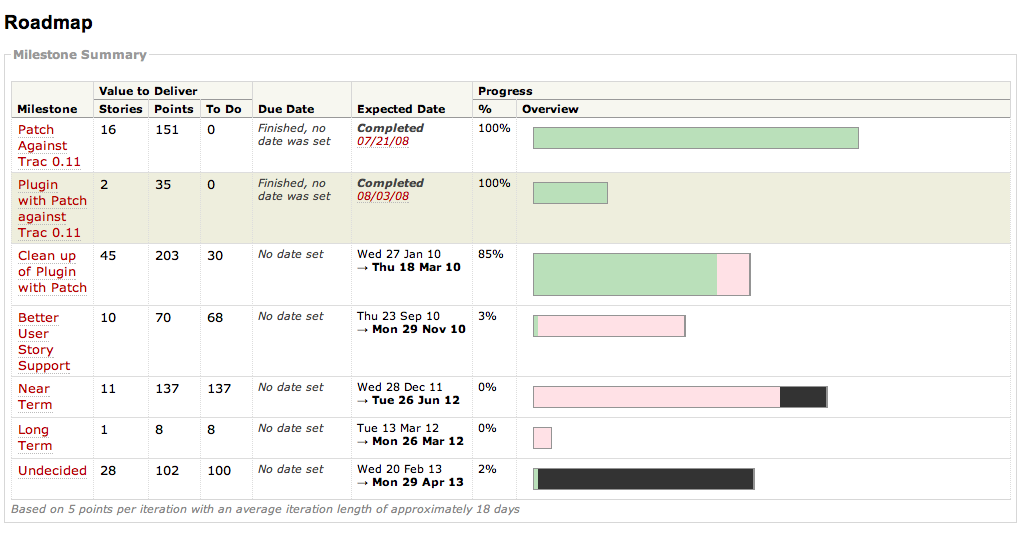
\includegraphics[width=110mm]{images/agile_trac_1.png}
  }
  \caption{Agile Trac}
\end{figure}

\begin{figure}[H]
  \centering
  \fbox{
    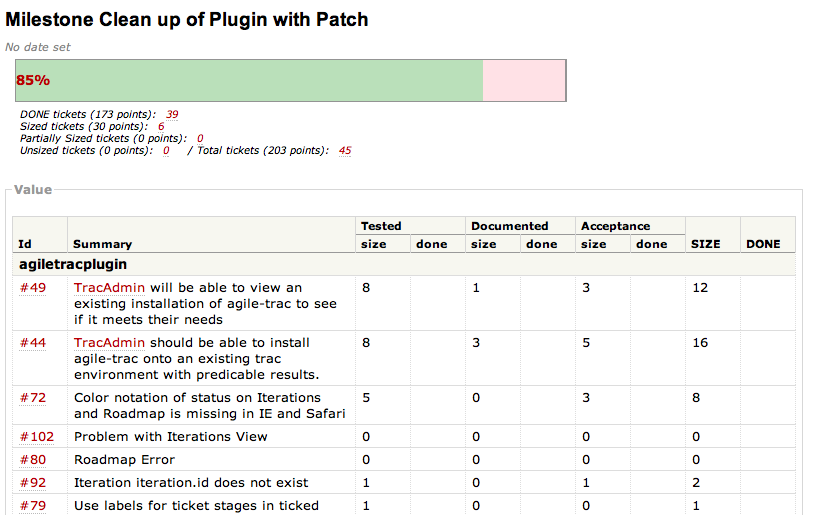
\includegraphics[width=110mm]{images/agile_trac_2.png}
  }
  \caption{Agile Trac}
\end{figure}

\item ScrumWorks

\item Rally
free / pro version - proprietario
integração com Eclipse =D
customização por widgets
usuarios com perfis diferentes (gerentes, dev, test, po)
graficos

\begin{figure}[H]
  \centering
  \fbox{
    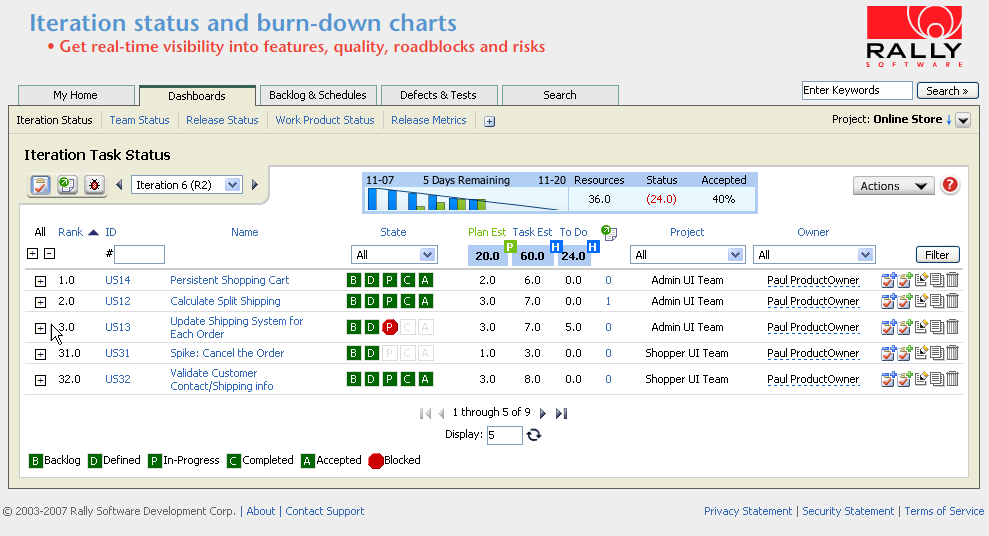
\includegraphics[width=110mm]{images/rally_1.png}
  }
  \caption{Rally}
\end{figure}

\begin{figure}[H]
  \centering
  \fbox{
    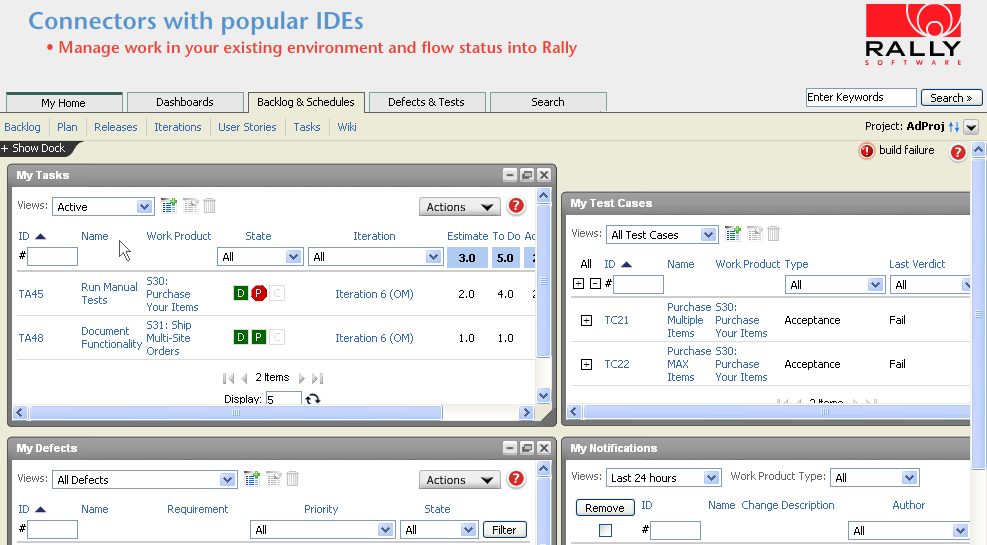
\includegraphics[width=110mm]{images/rally_2.png}
  }
  \caption{Rally}
\end{figure}

\begin{figure}[H]
  \centering
  \fbox{
    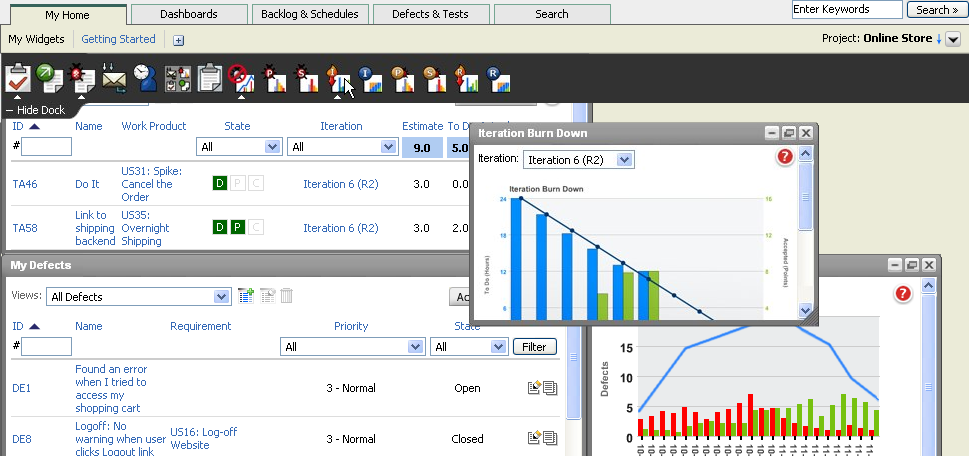
\includegraphics[width=110mm]{images/rally_3.png}
  }
  \caption{Rally}
\end{figure}

\item Mingle

\end{itemize}

\begin{sidewaystable}
	\begin{tabular}{|l|l|l|l|l|l|l|l}
		\hline
		\multicolumn{8}{|c|}{Aplicações similares} \\
		\hline
		 & PivotalTracker & Scrumy & ScrumNinja & Scrumd & VersionOne & BlueSoft & Mingle \\
		Gratuito & X & & & & & & \\
		OpenSource & - & & & & & & \\
		Graficos & X & & & & & & \\
		Estimativas & X & & & & & & \\
		Priorizacao & X & & & & & & \\
		Marcacao Horas & - & & & & & & \\
		Customizavel & & & & & & & \\
		Templates Metodologias & & & & & & & \\
		Templates Cartão & & & & & & & \\
		Personas & & & & & & & \\
		\hline
	\end{tabular}
\end{sidewaystable}


